\subsection{Puntos 4 y 5: análisis con fuentes reales}

Para los puntos 4 y 5 se modificó el flujograma de la práctica con el fin de reemplazar la fuente binaria aleatoria por datos provenientes de archivos reales. En lugar del bloque \texttt{Random Source}, se utilizó una fuente de archivo cuyos bytes fueron descompuestos en bits para alimentar la misma cadena de procesamiento usada en la generación de la señal binaria rectangular. De esta manera, fue posible comparar el comportamiento temporal y espectral de una secuencia aleatoria ideal frente a secuencias obtenidas a partir de información del mundo real.

\subsubsection{Punto 4: archivo de imagen \texttt{rana}}

Para este caso se empleó como entrada el archivo \texttt{rana}. La señal obtenida en el dominio del tiempo se presenta en la Figura~\ref{fig:p4_tiempo_rana}. A diferencia de una fuente puramente aleatoria, aquí la secuencia presenta una estructura asociada al contenido del archivo, lo que se refleja en una distribución no completamente uniforme de transiciones entre niveles. En consecuencia, aunque la señal sigue siendo rectangular y binaria, su comportamiento estadístico ya no corresponde al de una fuente IID ideal.

\begin{figure}[H]
    \centering
    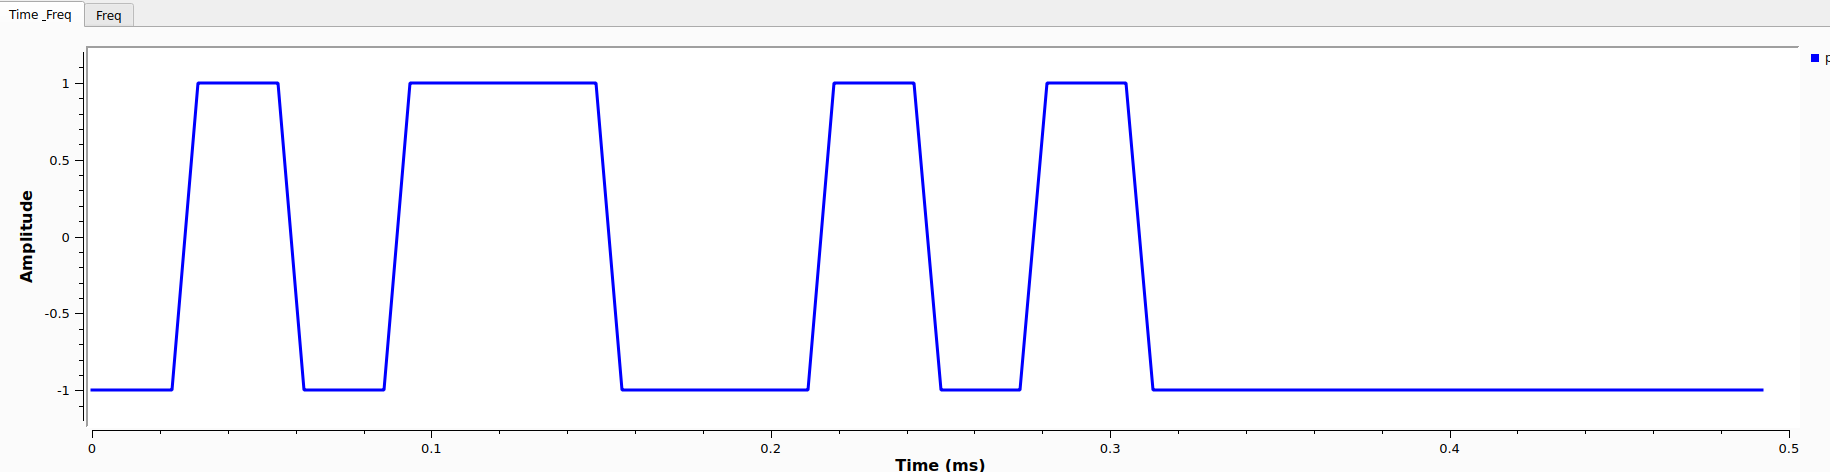
\includegraphics[width=0.86\linewidth]{imagenes/p4_tiempo_rana.png}
    \caption{Señal en el dominio del tiempo cuando la fuente de bits corresponde al archivo \texttt{rana}.}
    \label{fig:p4_tiempo_rana}
\end{figure}

La densidad espectral de potencia obtenida para esta señal se muestra en la Figura~\ref{fig:p4_psd_rana}. Se observa que la PSD conserva la envolvente general esperada para una señal binaria rectangular, pero su distribución energética no coincide exactamente con la de una fuente aleatoria ideal. Esto se debe a que los bits extraídos de una imagen real contienen redundancia y correlación, por lo que la energía no se reparte de forma completamente homogénea en frecuencia.

\begin{figure}[H]
    \centering
    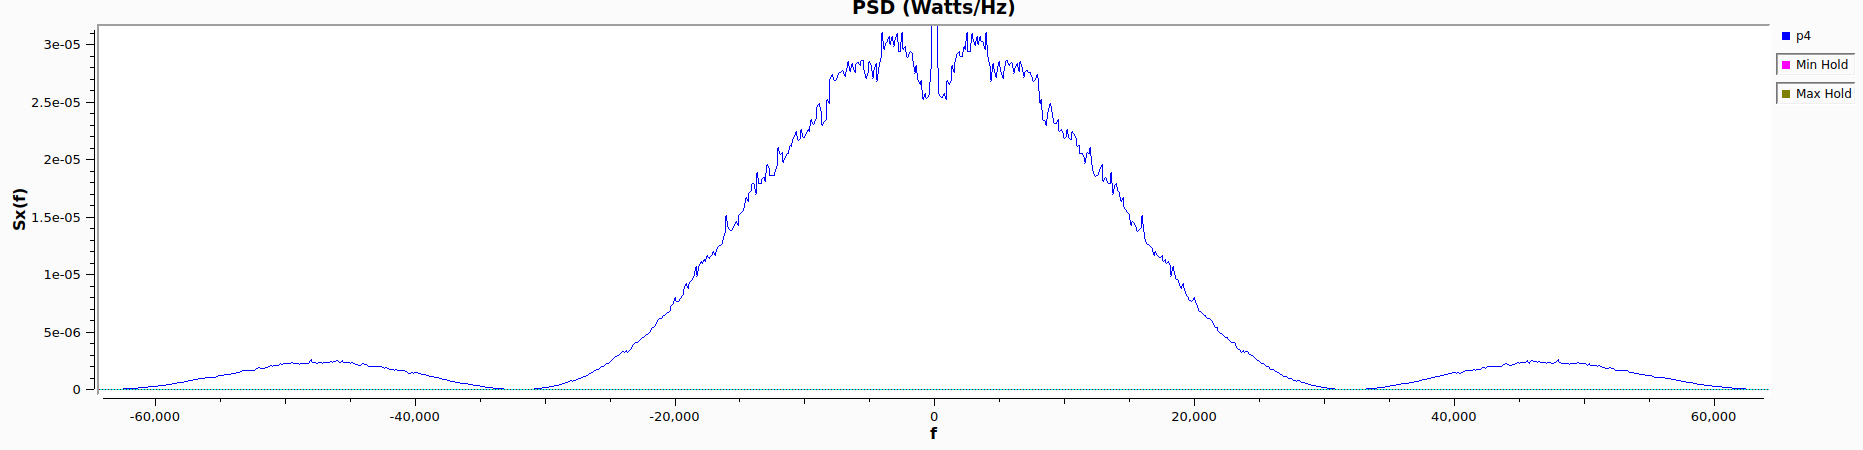
\includegraphics[width=0.86\linewidth]{imagenes/p4_psd_rana.png}
    \caption{PSD de la señal generada a partir del archivo \texttt{rana}.}
    \label{fig:p4_psd_rana}
\end{figure}

\subsubsection{Punto 5: archivo de audio \texttt{sonido}}

En el punto 5 se repitió el procedimiento anterior, pero utilizando el archivo \texttt{sonido} como fuente de datos. La señal temporal resultante se presenta en la Figura~\ref{fig:p5_tiempo_sonido}. En este caso también se conserva la forma rectangular de la señal, pero el patrón temporal observado responde a la estructura interna del audio digitalizado. Debido a la naturaleza del archivo, la secuencia de bits presenta una dependencia distinta a la de la imagen, lo cual modifica la estadística global de la señal.

\begin{figure}[H]
    \centering
    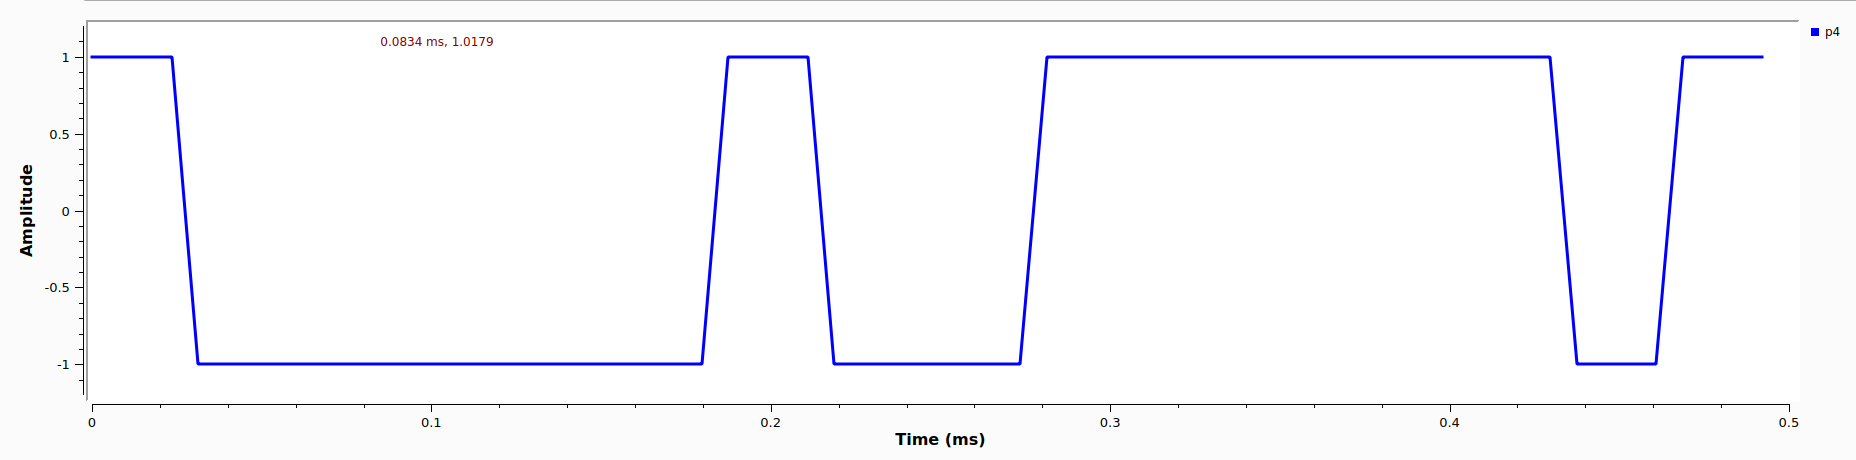
\includegraphics[width=0.86\linewidth]{imagenes/p5_tiempo_sonido.png}
    \caption{Señal en el dominio del tiempo cuando la fuente de bits corresponde al archivo \texttt{sonido}.}
    \label{fig:p5_tiempo_sonido}
\end{figure}

La PSD correspondiente se muestra en la Figura~\ref{fig:p5_psd_sonido}. Al compararla con la obtenida para el archivo de imagen, se evidencia que la forma espectral no es idéntica, aun cuando ambas señales se construyen finalmente como trenes rectangulares binarios. La diferencia se explica porque la fuente binaria ya no es aleatoria ideal, sino que depende del tipo de información almacenada en el archivo. En particular, los datos de audio suelen conservar cierta continuidad o correlación temporal entre muestras, lo cual influye en la distribución de energía del espectro.

\begin{figure}[H]
    \centering
    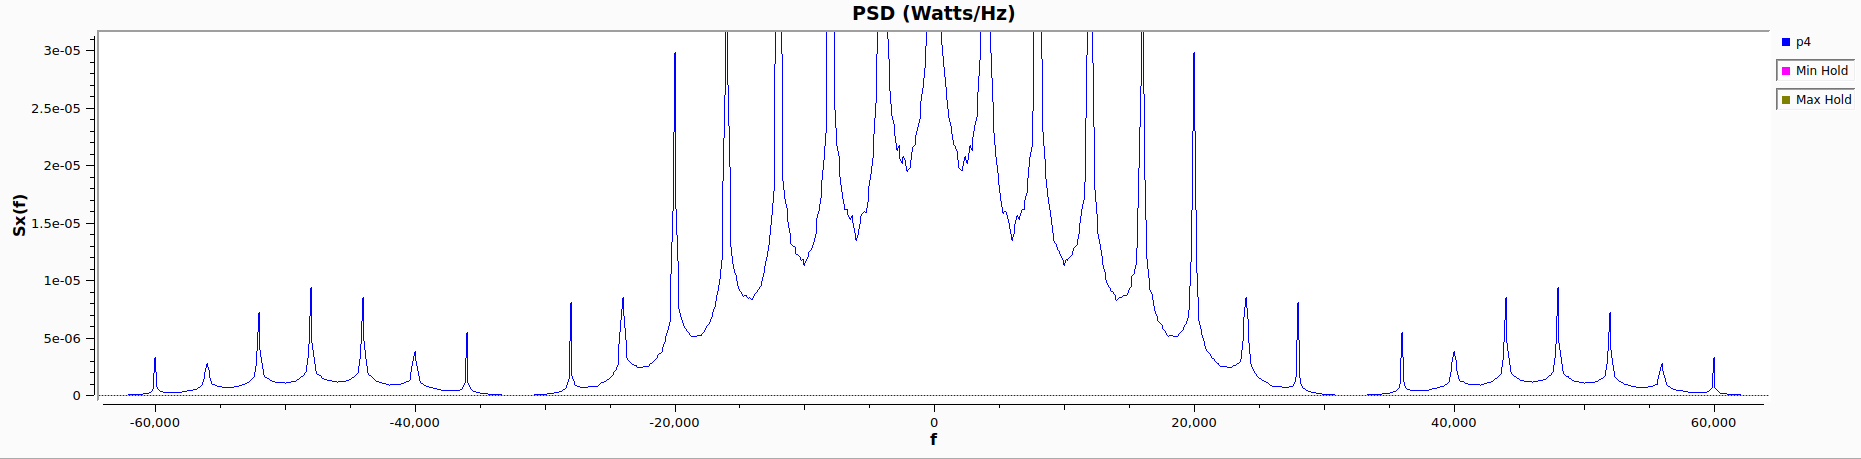
\includegraphics[width=0.86\linewidth]{imagenes/p5_psd_sonido.png}
    \caption{PSD de la señal generada a partir del archivo \texttt{sonido}.}
    \label{fig:p5_psd_sonido}
\end{figure}

\subsubsection{Caso complementario: efecto de aumentar \texttt{Sps} en la fuente de audio}

Como caso adicional, se analizó nuevamente la fuente \texttt{sonido} aumentando el número de muestras por símbolo a \(Sps=16\). La PSD obtenida se presenta en la Figura~\ref{fig:p5_psd_sonido_sps16}. Al incrementar \(Sps\), aumenta la frecuencia de muestreo de la señal rectangular, por lo que el espectro visible se extiende en un rango mayor de frecuencias. Sin embargo, la naturaleza espectral de la fuente no cambia: la señal sigue reflejando la estructura estadística propia del archivo de audio. Por tanto, variar \(Sps\) modifica la escala espectral y la forma en que se visualiza la PSD, pero no elimina la diferencia fundamental entre una fuente aleatoria ideal y una fuente real.

\begin{figure}[H]
    \centering
    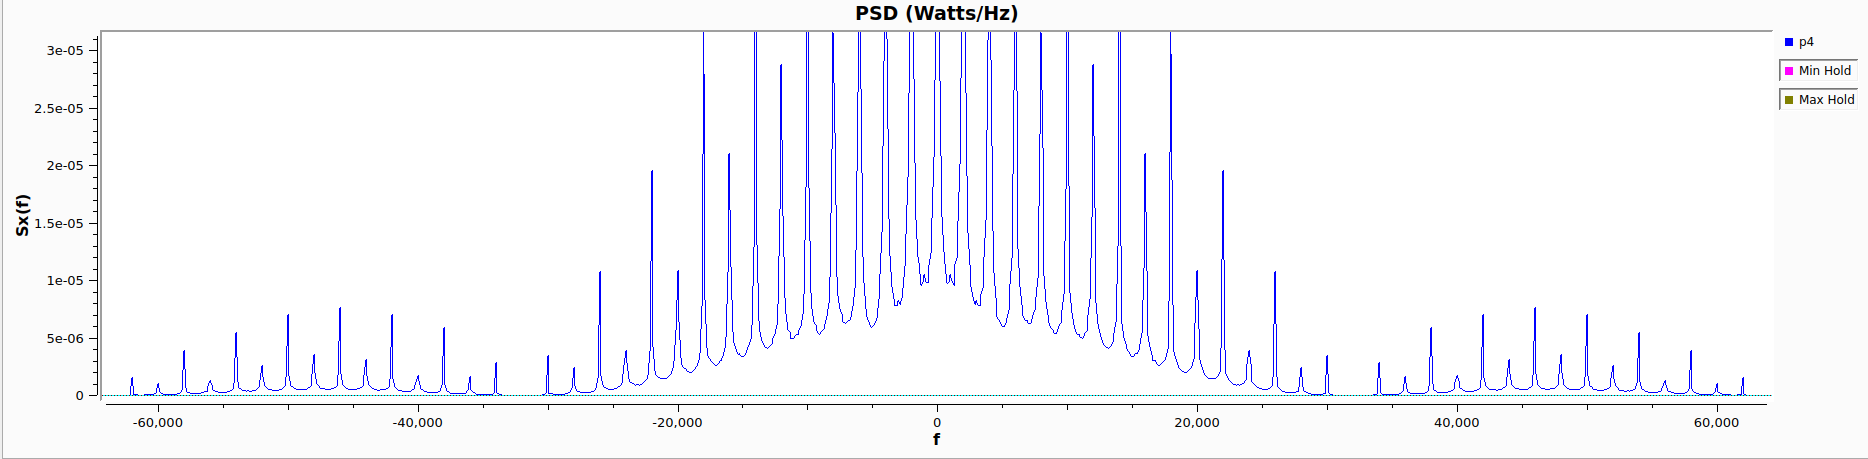
\includegraphics[width=0.86\linewidth]{imagenes/p5_psd_sonido_sps16.png}
    \caption{PSD de la señal obtenida a partir del archivo \texttt{sonido} usando \(Sps=16\).}
    \label{fig:p5_psd_sonido_sps16}
\end{figure}

En conjunto, los resultados de los puntos 4 y 5 muestran que la procedencia de los bits afecta de forma directa la apariencia temporal y espectral de la señal. Aunque en todos los casos la salida final corresponde a una señal binaria rectangular, el contenido estadístico de la fuente determina cómo se distribuye la energía en frecuencia. Por ello, una imagen y un audio, aun siendo almacenados digitalmente, no producen exactamente la misma PSD ni se comportan como una fuente binaria aleatoria ideal.